
% \counterwithin{figure}{section}
% \counterwithin{table}{section}

\chapter{Post-detection Barycentric Correction} \label{appen:barycenter}
We have developed a novel barycentric correction code specifically designed for high-spectral resolution \texttt{sigproc} filterbank products for technosignature searches \citep{Vishal_Bary}. The code uses the TEMPO routine to calculate relative velocity towards the observing targets at both locations, thus allowing for precise correction of the barycentric drift.

\begin{figure}[h]
    \centering
    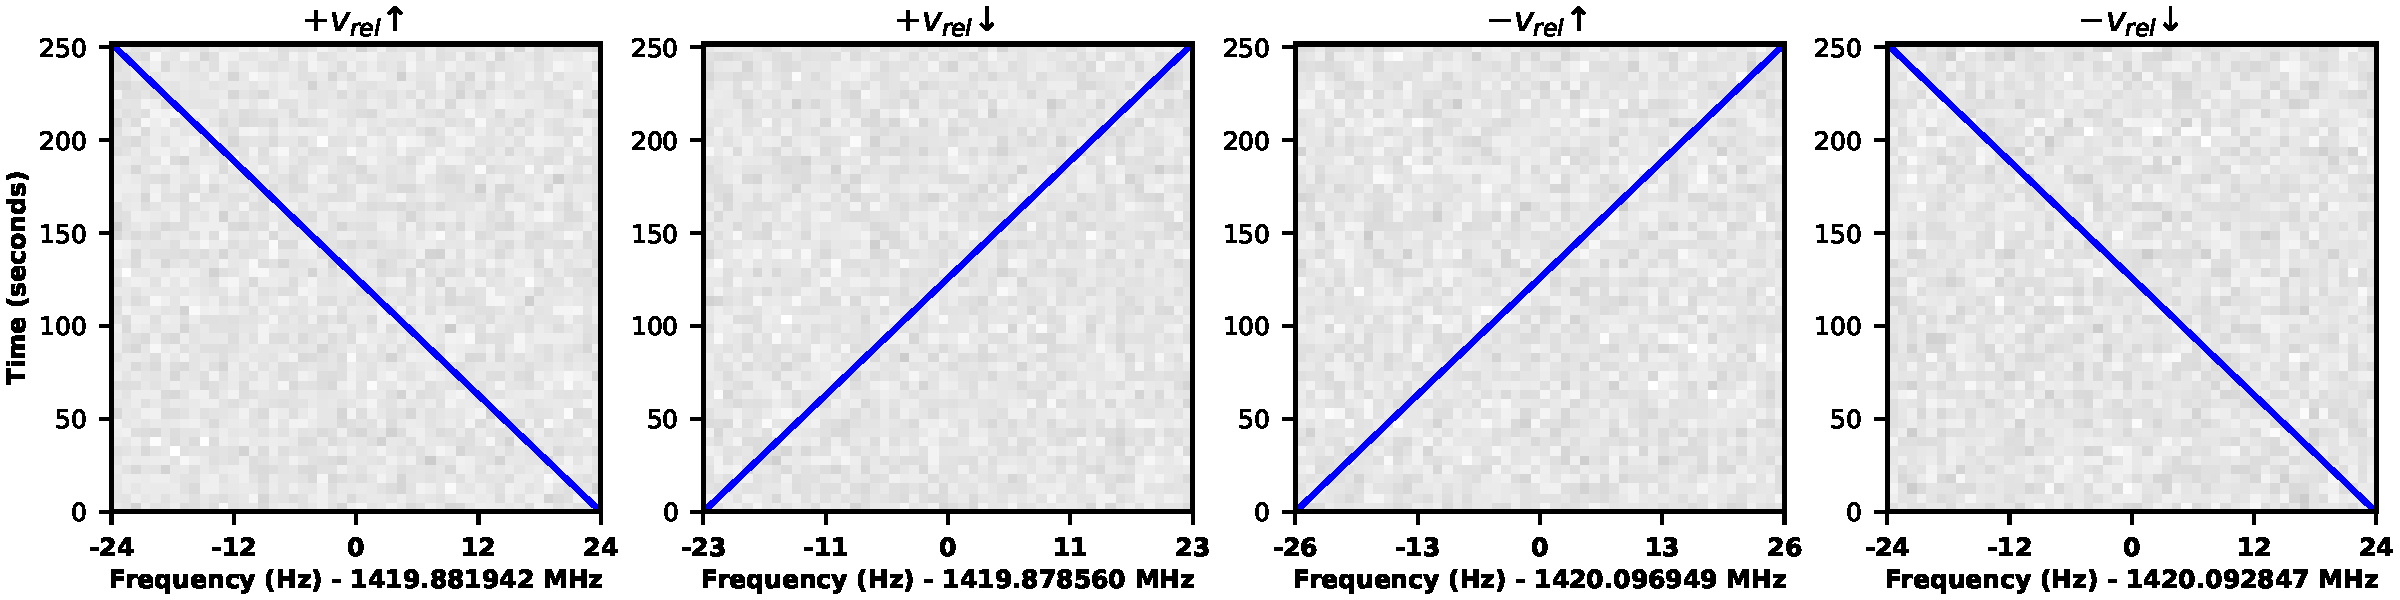
\includegraphics[scale=0.45]{SETI/figures/Barycentric_frequency_drift.pdf}
    \caption{Doppler drift of a narrowband signal in the topocentric observing frame at four different observing epochs. Simulated waterfalls with narrowband signals observed from the Irish LOFAR station towards the direction of TIC\,27677846 are shown for different times of the year in blue. The expected sign and direction of change of the relative velocity are labeled at the top of each plot. It is assumed that a hypothetical narrowband ETI signal is transmitted at a constant frequency of 1420\,MHz (with zero drift rate). As shown, the same signal is observed at different frequencies and drift rates depending on the sign and direction of change of the relative velocity at different epochs of observations. For instance, in the first panel, the relative velocity is positive and increases with observing time. Therefore, the observing frequency has been shifted to a lower frequency (as described by Equation \ref{eq:doppler}), and it continues to shift to even lower frequencies with time.}
    \label{fig:bary_simulated_drift}
\end{figure}
 
The Doppler shift caused by the relative motion between the transmitter and receiver will change over time as it is observed. Over a longer time frame, these shifts will exhibit a sinusoidal curve with a sidereal year period. Over a shorter time frame, the same pattern (superimposed on the yearly pattern) will be visible, but with a sidereal day period. Consequently, the relative velocity will change during the observation period, thereby altering the observed frequency of the received narrowband signal. This leads to a drift in the narrowband signal observed by the observer. Figure \ref{fig:bary_simulated_drift} displays examples of observed drifts at four different epochs for the same narrowband signal source observed from the same location. It is evident that if the relative velocity is positive and increasing with time (leftmost plot in Figure \ref{fig:bary_simulated_drift}), the signal, which is stationary in the barycentric frame, will drift towards lower frequencies as time progresses in the topocentric frame, as per Equation \ref{eq:doppler}.

\subsection{Algorithm outline}
Figure \ref{fig:example_filterbank_file} shows an example of how data is arranged in a filterbank file. For our case, we will assume that in a given filterbank file, frequency channels are in descending order with the first channel ($f_{1}$) having the highest frequency for each time sample. 
The goal of our tool is to shift every frequency channel from the observing frame to the actual emitted frequency frame after correcting for the barycentric relative velocity to remove any additional narrowband signal drift introduce by it. We aim to keep the first channel frequency of all the time samples the same in the barycentric frame also, thus relative shifts between spectras are needed to apply for each time sample corresponding to the inferred relative velocities. Our tool measures relative velocity at each time sample towards a given direction in the sky from a given telescope at the time of observations. Let's assume an observing scenario where $v_{rel}>0$. Following Equation \ref{eq:doppler}, we can state that the emitted frequency (or barycentric frequency) will be higher than the observed frequency. That means that observations stored in the first topocentric frequency channel correspond to higher barycentric frequency. Thus, this spectra needs to be shifted to higher frequency. If the relative velocity increases with time, the consecutive time sample's first channel barycentric frequency will be slightly higher than  the previous sample's first channel emitted frequency. Our tool thus shifts the spectra of each time sample towards higher frequency such that the first channel's emitted frequency matches across all time samples. 
Due to this shifts, we either replace empty channels at the edge of the spectra with zeros in case of squeeze or drop extra channels in case of expansion. 

As given in Equation \ref{eq:doppler}, the Doppler shifts are frequency-dependent, impacting higher frequencies more than lower frequencies. In other words, for spectra where frequencies are ordered from higher to lower frequency, the first channel will be shifted more compared to the last frequency channel. To compensate for this, we either expand or squeeze spectra as shown in Figure \ref{fig:spectra_expands_squeeze}. Figure \ref{fig:code_outline} outlines the logical flow of the code for a case of an input filterbank file with a descending order of frequency. By comparing Figure \ref{fig:bary_simulated_drift} and the code outline in Figure \ref{fig:code_outline}, we can consider one of the cases where the relative velocity is negative and increasing in absolute value with time. In this case, we need to shift consecutive spectra to lower and lower frequencies to match up their first frequency channel. Furthermore, for any negative relative velocity (either increasing or decreasing with time), we need to squeeze the individual spectra as shown in Figure \ref{fig:spectra_expands_squeeze}. Similarly, the same can be consider for the case of positive relative velocity. The code for this algorithm is publicly  available here\footnote{\url{https://github.com/gajjarv/BaryCentricCorrection}}.

\begin{figure}[h]
\centering
    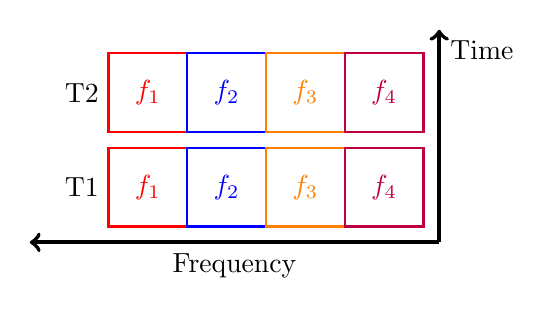
\begin{tikzpicture}
    \draw[->, line width=1.5pt] (4.2,-0.2) -- (-1,-0.2) node[midway,below] {Frequency};
    % Y axis
    \draw[->, line width=1.5pt] (4.2,-0.2) -- (4.2,2.5) node[anchor=north west] {Time};
        \draw[red,thick] (0,1.2) rectangle (1,2.2) node[midway] {$f_{1}$} ;
        \draw[blue,thick] (1,1.2) rectangle (2,2.2) node[midway] {$f_{2}$};
        \draw[orange,thick] (2,1.2) rectangle (3,2.2) node[midway] {$f_{3}$};
        \draw[purple,thick] (3,1.2) rectangle (4,2.2) node[midway] {$f_{4}$};
        \node[anchor=east] at (0,1.7) {T2};
        \draw[red,thick] (0,0) rectangle (1,1) node[midway] {$f_{1}$};
        \draw[blue,thick] (1,0) rectangle (2,1) node[midway] {$f_{2}$};
        \draw[orange,thick] (2,0) rectangle (3,1) node[midway] {$f_{3}$};
        \draw[purple,thick] (3,0) rectangle (4,1) node[midway] {$f_{4}$};
        \node[anchor=east] at (0,0.5) {T1};
    \end{tikzpicture}
    \caption{A typical filterbank file stores data in a time and frequency matrix format. Each row represents a sample, while each column represents a frequency channel for a given sample. Time is increasing from bottom to top while the frequency is increasing from right to left.}
    \label{fig:example_filterbank_file}
\end{figure}

\begin{figure}[h]
\centering
%    \subfloat{
    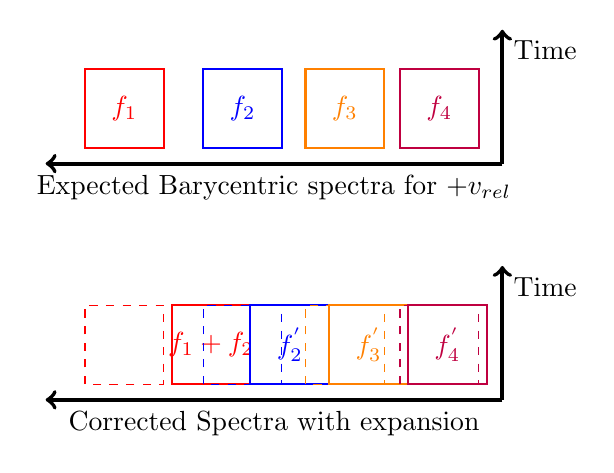
\begin{tikzpicture}
    \draw[->, line width=1.5pt] (4.8,-0.2) -- (-1,-0.2) node[midway,below] {Expected Barycentric spectra for $+v_{rel}$};
    % Y axis
    \draw[->, line width=1.5pt] (4.8,-0.2) -- (4.8,1.5) node[anchor=north west] {Time};
        \draw[red,thick] (-0.5,0) rectangle (0.5,1) node[midway] {$f_1$};
        \draw[blue,thick] (1.0,0) rectangle (2.0,1) node[midway] {$f_2$};
        \draw[orange,thick] (2.3,0) rectangle (3.3,1) node[midway] {$f_3$};
        \draw[purple,thick] (3.5,0) rectangle (4.5,1) node[midway] {$f_4$};
    \draw[->, line width=1.5pt] (4.8,-3.2) -- (-1,-3.2) node[midway,below] {Corrected Spectra with expansion};
    % Y axis
    \draw[->, line width=1.5pt] (4.8,-3.2) -- (4.8,-1.5) node[anchor=north west] {Time};
       \draw[red,dashed] (-0.5,-3) rectangle (0.5,-2) node[midway] {};
        \draw[red,thick] (0.6,-3) rectangle (1.6,-2) node[midway] {$f_1+f_2$};
        \draw[blue,dashed] (1,-3) rectangle (2,-2) node[midway] {};
        \draw[blue,thick] (1.6,-3) rectangle (2.6,-2) node[midway] {$f_2^{'}$};
        \draw[orange,thick] (2.6,-3) rectangle (3.6,-2) node[midway] {$f_3^{'}$};
        \draw[orange,dashed] (2.3,-3) rectangle (3.3,-2) node[midway] {};
        \draw[purple,thick] (3.6,-3) rectangle (4.6,-2) node[midway] {$f_4^{'}$};
        \draw[purple,dashed] (3.5,-3) rectangle (4.5,-2) node[midway] {};
    \end{tikzpicture}
%    }
%    \subfloat{
    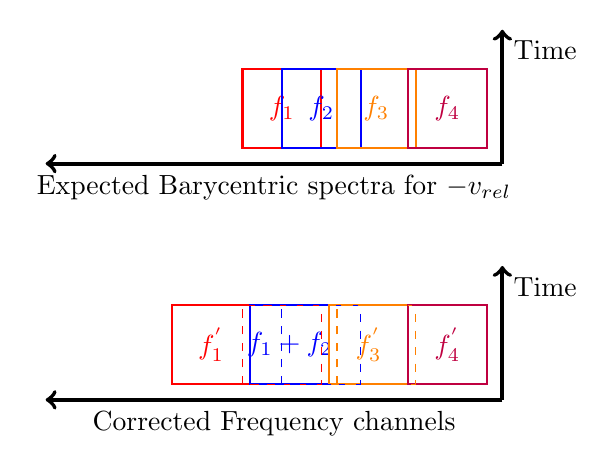
\begin{tikzpicture}
    \draw[->, line width=1.5pt] (4.8,-0.2) -- (-1,-0.2) node[midway,below] {Expected Barycentric spectra for $-v_{rel}$};
    % Y axis
    \draw[->, line width=1.5pt] (4.8,-0.2) -- (4.8,1.5) node[anchor=north west] {Time};
        \draw[red,thick] (1.5,0) rectangle (2.5,1) node[midway] {$f_{1}$};
        \draw[blue,thick] (2,0) rectangle (3,1) node[midway] {$f_{2}$};
        \draw[orange,thick] (2.7,0) rectangle (3.7,1) node[midway] {$f_{3}$};
        \draw[purple,thick] (3.6,0) rectangle (4.6,1) node[midway] {$f_{4}$};
    \draw[->, line width=1.5pt] (4.8,-3.2) -- (-1,-3.2) node[midway,below] {Corrected Frequency channels};
    % Y axis
    \draw[->, line width=1.5pt] (4.8,-3.2) -- (4.8,-1.5) node[anchor=north west] {Time};
        \draw[red,thick] (0.6,-3) rectangle (1.6,-2) node[midway] {$f_{1}^{'}$};
        \draw[blue,thick] (1.6,-3) rectangle (2.6,-2) node[midway] {$f_{1}+f_{2}$};
        \draw[orange,thick] (2.6,-3) rectangle (3.6,-2) node[midway] {$f_{3}^{'}$};
        \draw[purple,thick] (3.6,-3) rectangle (4.6,-2) node[midway] {$f_{4}^{'}$};
        \draw[red,dashed] (1.5,-3) rectangle (2.5,-2) node[midway] {};
        \draw[blue,dashed] (2,-3) rectangle (3,-2) node[midway] {};
        \draw[orange,dashed] (2.7,-3) rectangle (3.7,-2) node[midway] {};
        \draw[purple,dashed] (3.6,-3) rectangle (4.6,-2) node[midway] {};
    \end{tikzpicture}
%    }
    \caption{These plots depict the expected spectra at their respective barycentric frequencies and the spectra after the correction for barycentric relative velocity. Each plot represents a single spectrum, where the frequency increases from right to left. (a) In the case of $+v_{rel}$, the first channel of the topocentric spectra is shifted to a higher barycentric frequency compared to the last topocentric spectra channel, which causes an expansion of the spectra. If two consecutive channels move farther away from each other (shown as $f_1$ and $f_2$) by more than half the channel width, an additional channel is added in between, which is the summation of these two channels. Extra channels at the edge of the spectra are dropped. (b) In the case of $-v_{rel}$, the first channel of the topocentric frequency is shifted to a lower barycentric frequency relative to the last topocentric spectra channel, which causes a squeeze in the spectra. If two consecutive frequency channels shift closer to each other by more than half a channel width, these channels are added together and an extra channel is added at the end containing zeros. The bottom spectra in each plot illustrate these expansion and squeeze effects after correction are applied from the code. 
    }
    \label{fig:spectra_expands_squeeze}
\end{figure}

\begin{figure}[h]
    \centering
\begin{tikzpicture}[node distance=2cm]
% Define nodes
\tikzstyle{startstop} = [rectangle, rounded corners, minimum width=3cm, minimum height=1cm,text centered, draw=black, fill=red!30]
\tikzstyle{io} = [rectangle, minimum width=3cm, minimum height=1cm, text centered, draw=black, fill=blue!30]
\tikzstyle{process} = [rectangle, minimum width=3cm, minimum height=1cm, text centered, draw=black, fill=orange!30]
\tikzstyle{decision} = [diamond, minimum width=3cm, minimum height=1cm, text centered, draw=black, fill=green!30]
\tikzstyle{arrow} = [thick,->,>=stealth]
    % Draw nodes
    \node (start) [startstop] {Input filterbank in topocentric frame};
    \node (dec1) [decision, below of=start] {\large $v_{rel}>0$};
    \node (dec2) [decision, left of=dec1, xshift=-2cm, yshift=-2cm] {\large $|v_{rel}|\uparrow?$};
    \node (proc1) [process, below of=dec2, xshift=-2cm, yshift=-0.0cm] {Shift to higher frequency};
    \node (proc2) [process, below of=dec2, xshift=2cm, yshift=-0.0cm] {Shift to lower frequency};
    \node (proc3) [process, below of=dec2, yshift=-1.5cm] {Expand};
    \node (dec3) [decision, right of=dec1, xshift=2cm, yshift=-2cm] {\large $|v_{rel}|\uparrow?$};
    \node (proc4) [process, below of=dec3, xshift=-2cm, yshift=-0.0cm] {Shift to lower frequency};
    \node (proc5) [process, below of=dec3, xshift=2cm, yshift=-0.0cm] {Shift to higher frequency};
    \node (proc6) [process, below of=dec3, yshift=-1.5cm] {Squeeze};
    \node (stop) [startstop, below of=dec1, yshift=-5cm] {Output filterbank in barycentric frame};
    % Draw arrows
    \draw [arrow] (start) -- (dec1);
    %\draw [arrow] (dec1) -- node[anchor=east] {yes} (dec2);
    \draw [arrow] (dec1.west) -| node[anchor=east] {Yes} (dec2.north);
    \draw [arrow] (dec2.west) -| node[anchor=east] {Yes} (proc1.north);
    \draw [arrow] (dec2.east) -| node[anchor=west] {No} (proc2.north);
    \draw [arrow] (proc1.south) |- (proc3.west);
    \draw [arrow] (proc2.south) |- (proc3.east);  
    \draw [arrow] (dec1.east) -| node[anchor=west] {No} (dec3.north);
    \draw [arrow] (dec3.west) -| node[anchor=east] {Yes} (proc4.north);
    \draw [arrow] (dec3.east) -| node[anchor=west] {No} (proc5.north);
    \draw [arrow] (proc4.south) |- (proc6.west);
    \draw [arrow] (proc5.south) |- (proc6.east);
    \draw [arrow] (proc6.south) |- (stop);
    \draw [arrow] (proc3.south) |- (stop);
    %\draw [arrow] (dec2) -- (stop);
\end{tikzpicture}
\caption{An outline of the post-detection barycentric correction algorithm for an input filterbank file in \texttt{sigproc}  format. For this case, the input filterbank file has a descending order in frequency, and $v_{rel}$ represents the relative velocity between the transmitter and observer. The algorithm considers two cases depending on whether the relative velocity is positive or negative, which indicates whether the source is moving away from or towards the observer, respectively. Each of these cases is further divided into two where the absolute value of the relative velocity can either increase or decrease, requiring the spectra to be shifted to either the higher or lower frequency end. 
For all cases with $+v_{rel}$, each spectra is expanded, and for $-v_{rel}$, each spectra is squeezed, as shown in Figure \ref{fig:spectra_expands_squeeze}. 
The code then writes each of these spectra into another \texttt{sigproc}  filterbank file, which will have each channel frequency closely corrected to the barycentric frame of reference.}  
\label{fig:code_outline}
\end{figure}


\section{Sensitivity of the Survey across the HBA}
\label{SEC2:A2}
As previously stated the high band antenna spans from 110 - 190 MHz. The system temperature across the band significantly, which reduces the sensitivity of LOFAR at the lower end of the band-pass (see. \Cref{fig:Cumulative_EIRP_plots}). Calculation of $T_{sys}$ and consquently SEFD follows a modified method as outlined in \S~3.3 of \cite{David-RRAT}. The method differs in the calculation of $T_{sky}$ as this is pointing dependent. This study uses the LWA1 Low Frequency Sky Survey \citep{LWA-survey} for sensitivity analysis. We calculate system equivalent flux density (SEFD; Jy) as follows, 

\begin{equation}
    \text{SEFD} = \frac{2 T_{\text{sys}} k_b}{A_e}
\end{equation}

Where $k_b$ is the Boltzmann constant and $A_e$ is the effective collecting area of a single staion HBA. EIRP is then consequently calculated using \Cref{Eq:EIRP}.

\begin{table}[!ht]
    \centering
    \begin{tabular}{l|ccccccccc}
    \hline
        \textbf{Frequency (MHz)} & 110 & 120 & 130 & 140 & 150 & 160 & 170 & 180 & 190 \\ \hline
        $\bar T_{\text{sys}}$ (K) & 1305.073 &  1051.633 &   862.204 &   717.304 &  604.260 &  514.594 &  442.408 &  383.552 &  335.019 \\
        $\overline{\text{SEFD}}$ (Jy) &2148.125 &  1730.967 &  1419.171 &  1180.668 &  994.601 &  847.011 &  728.195 &  631.320 &  551.435 \\
        $\overline{\text{EIRP}}$ (W) & 17.273 &    17.179 &    17.092 &    17.011 &   16.937 &   16.866 &   16.801 &   16.738 &   16.679 \\ 
        $\text{EIRP}_\text{median}$ (W) & 17.235 &    17.141 &    17.054 &    16.974 &   16.899 &   16.829 &   16.763 &   16.701 &   16.642 \\
         ${\text{EIRP}_\text{max}}$ (W)& 19.628 &    19.537 &    19.454 &    19.377 &    19.304 &   19.237 &   19.173 &   19.112 &   19.055 \\ 
        ${\text{EIRP}_\text{min}}$ (W)&12.627 &    12.627 &    12.627 &    12.627 &   12.627 &   12.627 &   12.627 &   12.627 &   12.627 \\
        K1 detectable (\%) &   25.497 &    34.493 &    43.910 &    52.859 &   60.644 &   66.968 &   71.969 &   75.887 &   79.032 \\
        Earth detectable (\%) & 14.659 &    20.613 &    27.730 &    35.694 &   43.908 &   51.781 &   58.826 &   64.739 &   69.612 \\\hline \hline 
    \end{tabular}
    \caption{Statistics on sensitivity across the HBA band. The K1 and Earth detectable values represent the percentage of the target sample that are detectable.}
\end{table}
